\documentclass[]{article}
%----------------- PAKETE INKLUDIEREN ----------------- %

\usepackage{geometry} % Packet für Seitenrandabständex und Einstellung für Seitenränder
\usepackage[ngerman]{babel} % deutsche Silbentrennung

\usepackage{booktabs} %entzerrt die Tabellenzeilen und bietet verschieden dicke Unterteilungslinien
\usepackage{longtable} % Tabellen können sich nicht über mehrere Seiten 
\usepackage{graphicx} % kann LaTeX Grafiken einbinden

%\usepackage[applemac]{inputenc} % Umlaute unter Mac werden automatisch gesetzt
\usepackage[T1]{fontenc} % Zeichenencoding
\usepackage[utf8]{inputenc}
\usepackage{lmodern} % typographische Qualität 
\frenchspacing % Schaltet den zusätzlichen Zwischenraum ab
\usepackage{fix-cm}
\usepackage{hyperref} % verwandelt alle Kapitelüberschriften, Verweise aufs Literaturverzeichnis und andere Querverweise in PDF-Hyperlinks
\usepackage{color}
\usepackage{url}

\usepackage[nottoc]{tocbibind}
\usepackage{subfigure}
\usepackage{float}

% für Listings
\usepackage{listings}
\lstset{numbers=left, numberstyle=\tiny, numbersep=5pt, stepnumber=4, keywordstyle=\color{black}\bfseries\itshape, stringstyle=\ttfamily,showstringspaces=false,basicstyle=\footnotesize,captionpos=b}
\lstset{language=java}
%Todos
\usepackage{todonotes} % to erase all comments by adding [disable]

%opening
\title{Ausarbeitung zu Chaos und Faktale Praktikum 1}
\author{Jannis Priesnitz\space \textperiodcentered \space Margarethe Dziendziel}

\begin{document}

\maketitle
\begin{center}

\end{center}
\section{Teilaufgabe 3}
Die Ausgabe des Endergebnisses ist gleich, da die Berechnungsvorschrift das gleiche Ergebnis liefert. 

Um sich dies klar zu machen ist es hilfreich zunächst die Ergebnismenge für eine Position zu analysieren: Diese kann durch die "`Modulo 2"' Operation der Jacobimatrix nur 0 und 1 annehmen. Die Berechnungsvorschrift des LUT-Automaten liefert per Definition ebenfalls nur 0 und 1.

Schaut man sich nun an, wann ein Eintrag in der Jacobimatrix ungerade wird, so erkennt man, dass dies der Fall ist, wenn die Felder, aus denen das Ergebnis berechnet wird je einen ungeraden und einen geraden Eintrag enthalten (auf den Beweis soll an dieser Stelle verzichtet werden). Somit entsteht in den Zellen [1, i] und [n,n] wobei n = Anzahl der Iterationsschritte eine 1, also ein ungerader Wert. 

Analog kann man im LUT ebenfalls die Generierung der beiden 1-Reihen beobachten, die sich direkt aus der Berechnungsvorschrift ableiten lässt. 

Nun ist es naheliegend, dass Bereiche mit geraden Werten "`ausdehnen"', da je zwei gerade und ungerade Werte einen geraden Wert erzeugen (gut erkennbar z.B. an Iteration 4 und 8). Diese Ausdehnung wird jedoch nicht endlos fortgeführt, sondern zunehmend von ungeraden Werten "`gestört"', die durch die Einsen am Rande generiert werden und mit steigender Anzahl Iterationen in Richtung Mitte vordringen. Haben diese eine Zeile komplett gefüllt "`kippen"' in der nächsten Iteration alle Werte ins gerade und die Prozess startet von neuem. Dies wiederholt sich im Kleinen, wie im Großen wodurch die gesehenen, fraktalen Strukturen entstehen.

\section{Teilaufgabe 4}
Die vom Ursprung\footnote{Wir definieren hier den Ursprung oben links.} aus verlaufende Diagonale enthält immer die Farbe schwarz. Dies lässt sich einfach dadurch begründen, dass für die Indizes $i$ und $j$ gilt $i = j$. Da außerdem leicht zu sehen ist, dass $i \& i = i$ gilt kann kein Index (mit Ausnahme der $0$) $0$ sein.

Die andere Diagonale enthält ebenfalls immer die Farbe schwarz. Dies lässt sich leicht erklären, wenn man sich klar macht, dass auf dieser Diagonalen ausschließlich die Werte 1, 2 und Vielfache von 2 vorkommen, die $\leq 256$ sind. Dabei kommt die 256 genau ein mal bei $i = 255$ und $j = 256$ vor, die 128 zwei mal bei $i = 127, j = 384$ und $i = 383, j = 128$ usw. Dies lässt sich durch einen Blick auf die binäre Repräsentation der Zahlen erkennen. 
\section{Teilaufgabe 5}
Anmerkung: Es wurde nur Teilaufgabe b gelöst und daher hier auch nur dieser Teil näher beschrieben.
\subsection{Teilaufgabe b}
Das Problem bei dieser Aufgabe ist der Überlauf der bei normalen 32 Bit Intergern auftritt. Durch diesen wird die Modulorechnung so verfälscht, dass das in der Aufgabe genannte Pixelrauschen entsteht. 
Die Teilaufgabe wurde durch Verwendung der bereitgestellten Bibliothek für große Zahlen gelöst. Durch die beliebige Größe von Intergern tritt nun auch bei großen Zahlen keine Überlauf mehr auf und die Modulorechnung ergibt das richtige Ergebnis.
\begin{figure}[H]
	\subfigure[modulo 2]{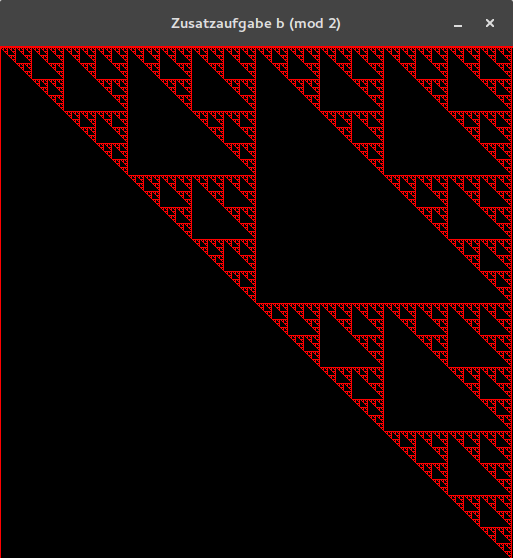
\includegraphics[width=0.50\textwidth]{Img/Zb_mod2.png}}
	\subfigure[modulo mit 2\textsuperscript{3} (8)]{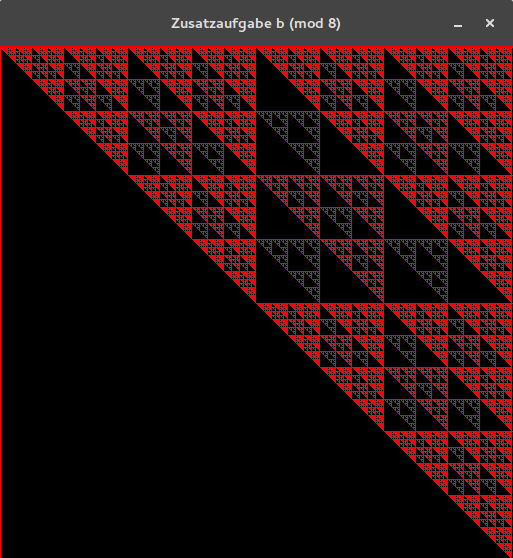
\includegraphics[width=0.50\textwidth]{Img/Zb_mod8.png}}
	\subfigure[modulo mit der Primzahl 7]{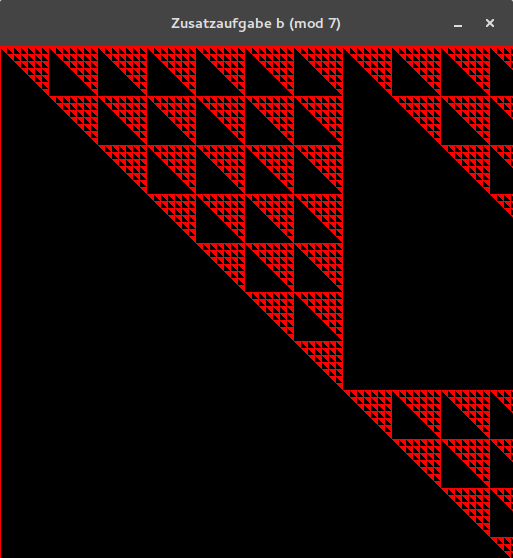
\includegraphics[width=0.50\textwidth]{Img/Zb_mod7.png}}
	\subfigure[modulo 10]{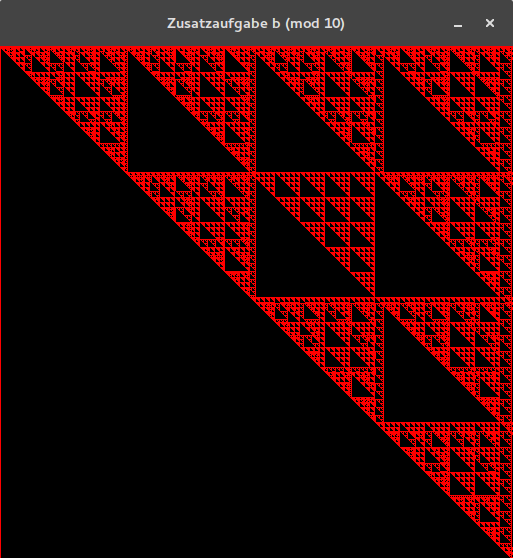
\includegraphics[width=0.50\textwidth]{Img/Zb_mod10.png}}
	\caption{Zusatzaufgabe b}
\end{figure}
\end{document}
